\part{Matlab programming I}
\section{Introduction}
\subsection*{General}
\begin{frame}[label=contents_prog1]
  \frametitle{Today's outline}
  \mode<beamer>{
    \only<1>{\tableofcontents}
  }
  \only<2>{\tableofcontents[currentsection]}
\end{frame}

\begin{frame}
 \frametitle{Why should you learn something about programming?}
 \begin{itemize}[<+->]
  \item Scientific techniques depend in an increasing fashion upon computer programs and simulation methods
  \item Knowledge of programming allows you to automate routine tasks 
  \item Ability to understand algorithms by inspection of the code 
  \item Learn to think by dissecting a problem into smaller bits 
 \end{itemize}\vskip2em
 \begin{columns}
  \column<1->{0.23\textwidth}
  \tikz\node[circle,draw,very thick,maincolor,
           text=white,minimum size=\columnwidth,
           path picture={
               \node at (path picture bounding box.center){
                   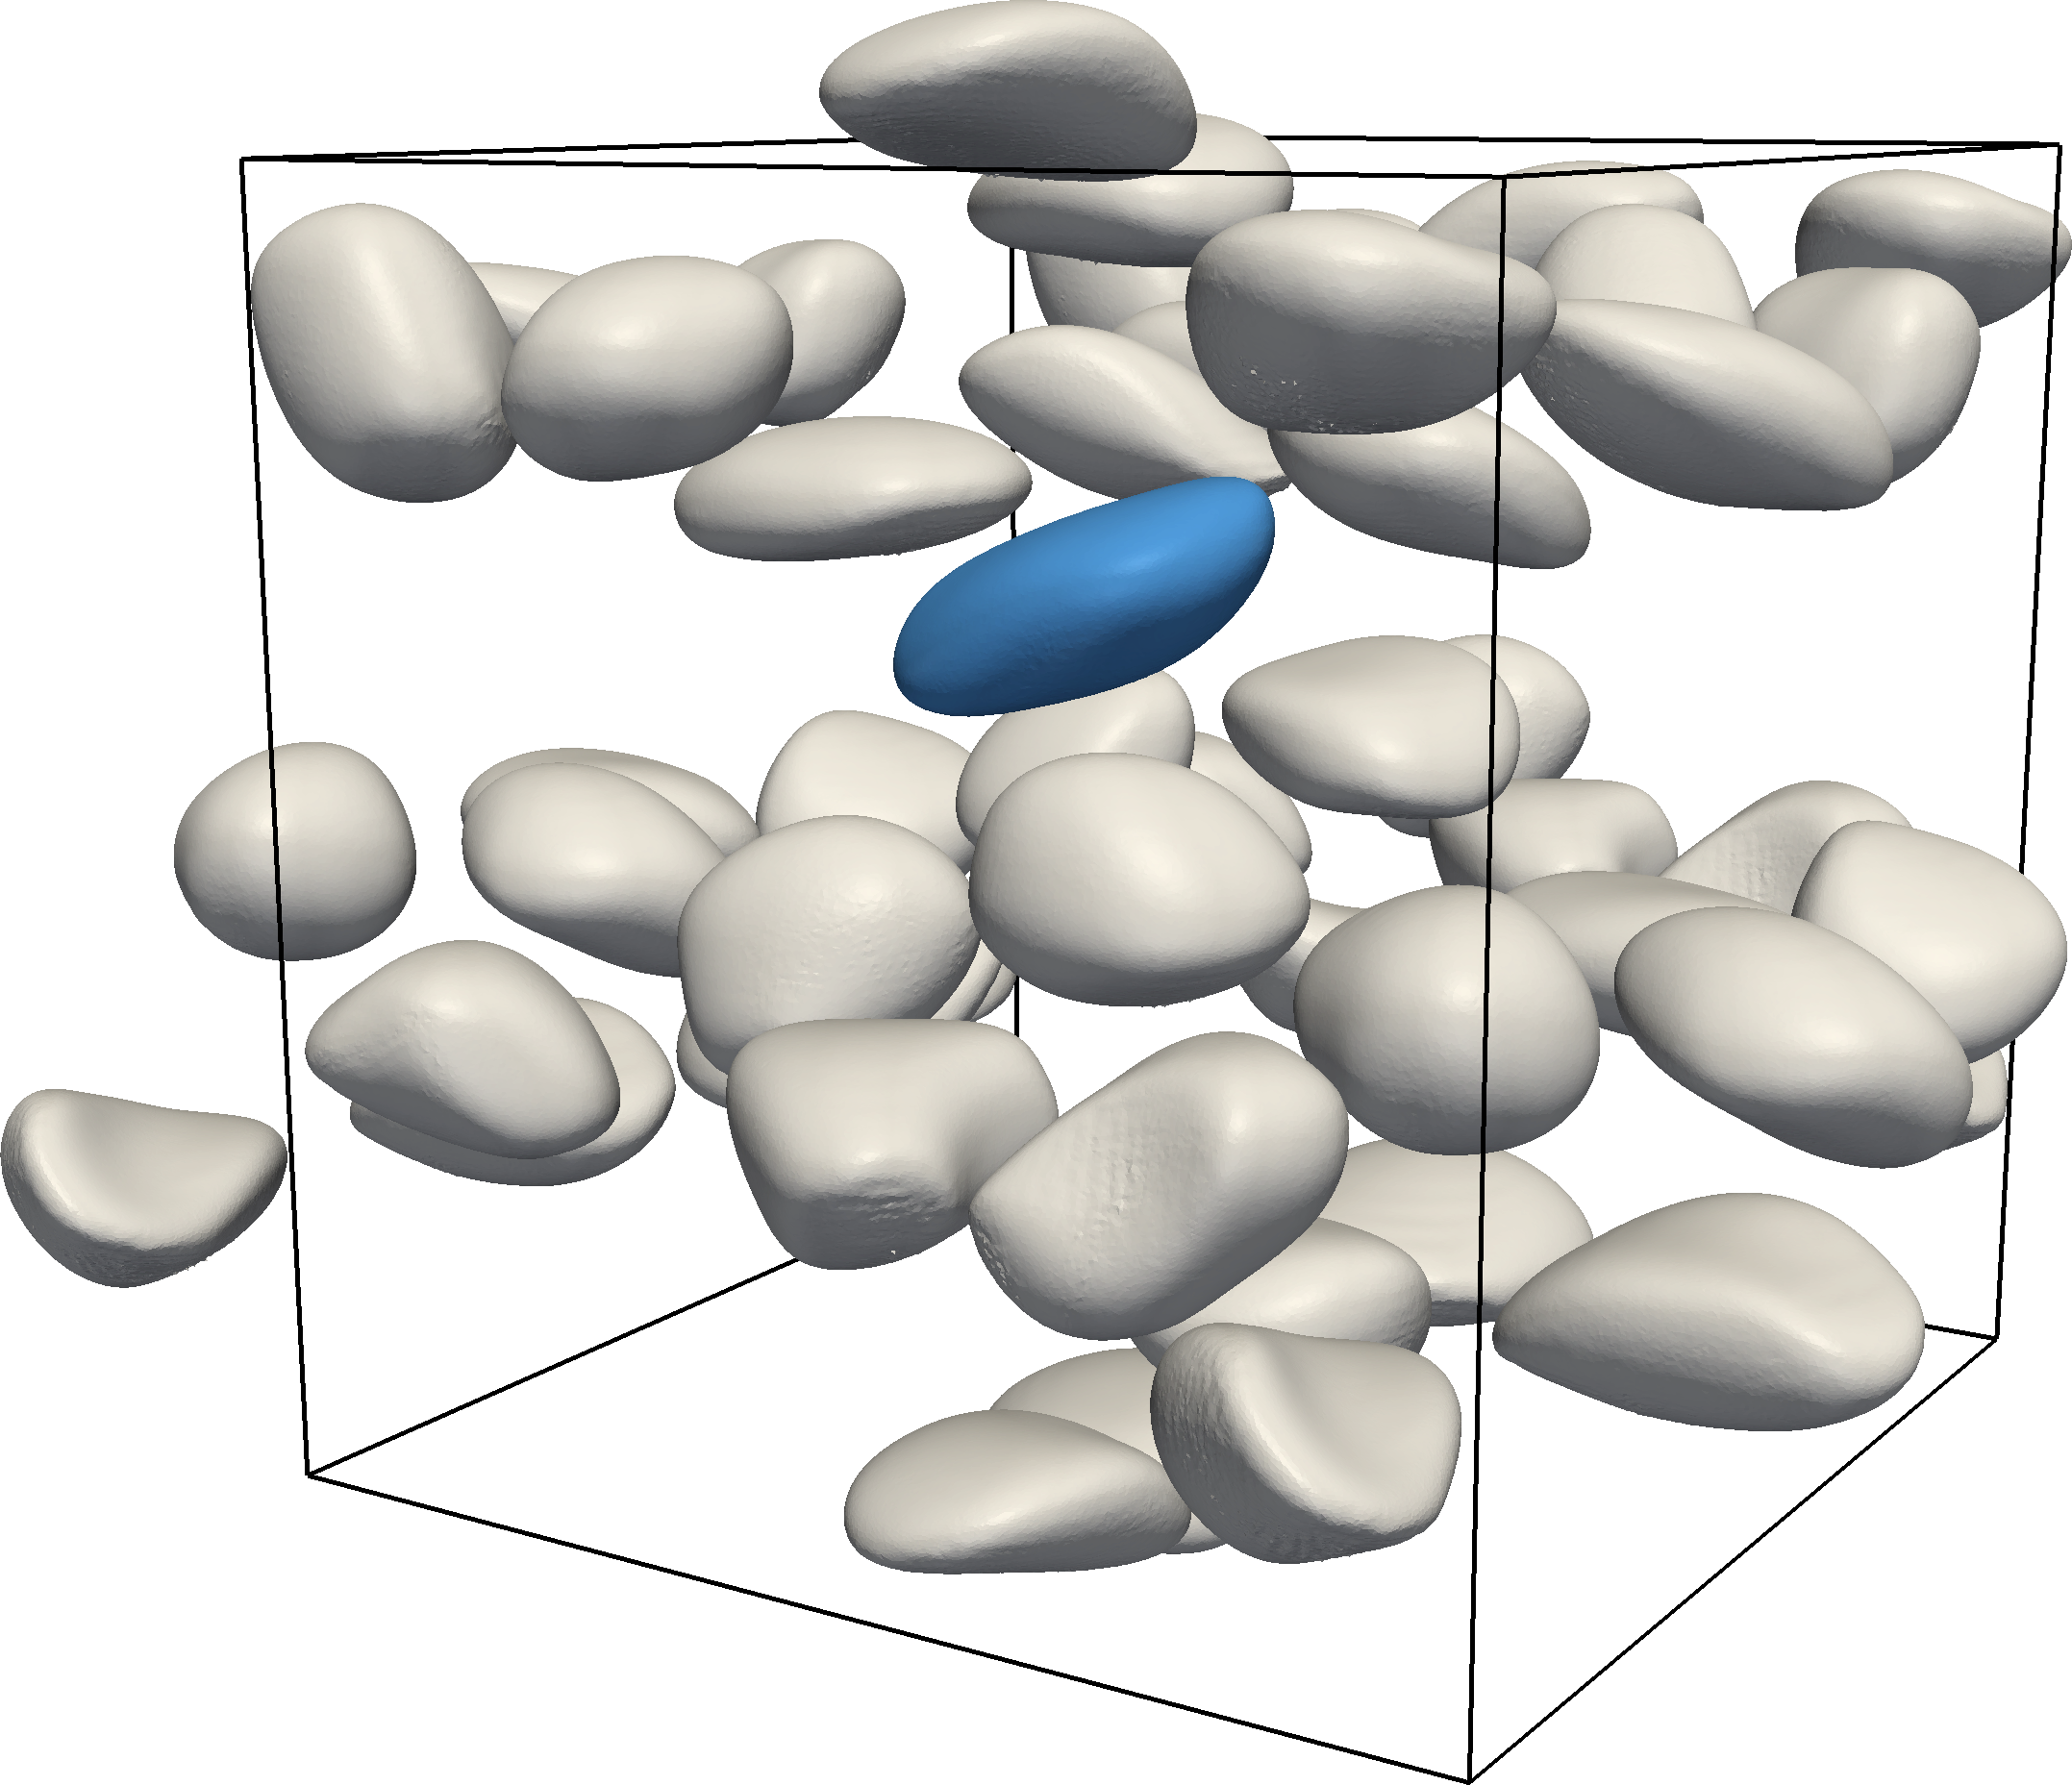
\includegraphics[width=\columnwidth]{sim1.png}
               };
           }]{};
  \column<2->{0.23\textwidth}
  \tikz\node[circle,draw,very thick,maincolor,
           text=white,minimum size=\columnwidth,
           path picture={
               \node at (path picture bounding box.center){
                   
\includegraphics[width=1.1\columnwidth]{automate.jpg}
               };
           }]{};
  \column<3->{0.23\textwidth}
  \tikz\node[circle,draw,very thick,maincolor,
           text=white,minimum size=\columnwidth,
           path picture={
               \node at (path picture bounding box.center){
                   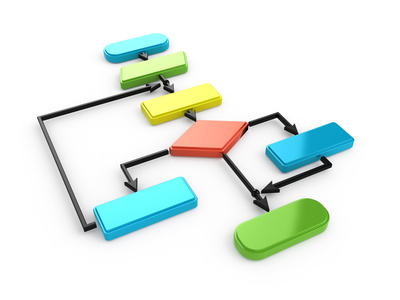
\includegraphics[width=1.2\columnwidth]{algorithm.jpg}
               };
           }]{};
  \column<4>{0.23\textwidth}
  \tikz\node[circle,draw,very thick,maincolor,
           text=white,minimum size=\columnwidth,
           path picture={
               \node at (path picture bounding box.center){
                   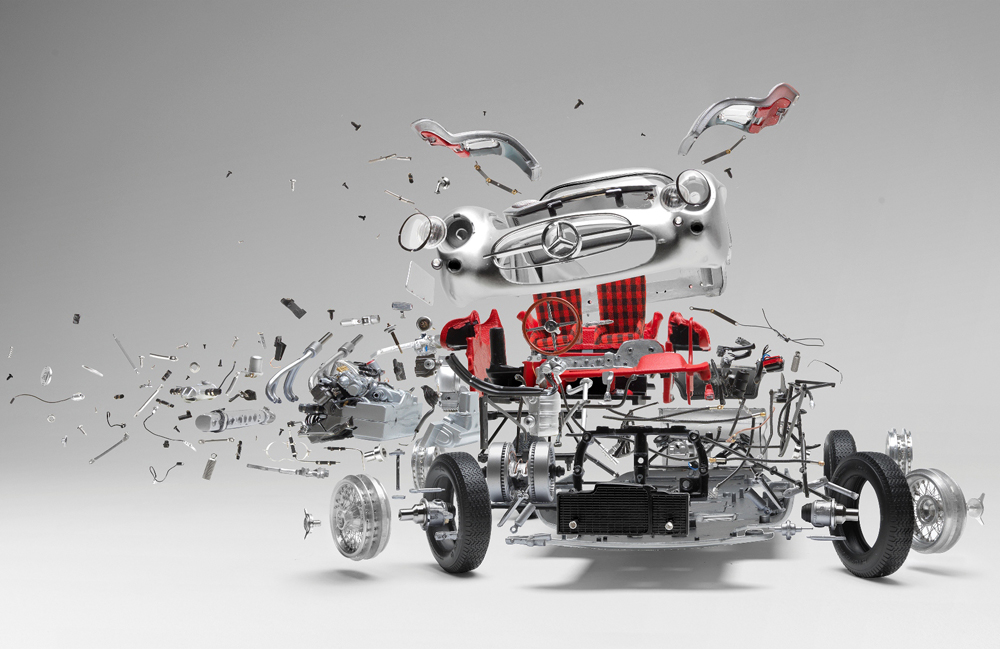
\includegraphics[width=1.5\columnwidth]{dissect.jpg}
               };
           }]{};
 \end{columns}
\end{frame}

\begin{frame}
 \frametitle{Introduction to programming}
 \begin{block}{What is a program?}
  \emph{A program is a sequence of instructions that is written to perform a certain task on a computer.} % SOURCE http://www.greenteapress.com/thinkpython/html/thinkpython002.html
  \end{block}
  \begin{itemize}
    \item The computation might be something mathematical, a symbolic operation, image analysis, etc.%such as solving a system of equations or finding the roots of a polynomial
    % \item It can also be a symbolic computation, such as searching and replacing text in a document 
    % \item A program may even be used to compile another program
    % \item A program consists of one or more \emph{algorithms}
  \end{itemize}
  \begin{block}{Program layout}
    \begin{enumerate}
        \item Input (Get the radius of a circle)
        \item Operations (Compute and store the area of the circle)
        \item Output (Print the area to the screen)
    \end{enumerate}
  \end{block}
\end{frame}

\begin{frame}
\frametitle{Versatility of Matlab}
\centering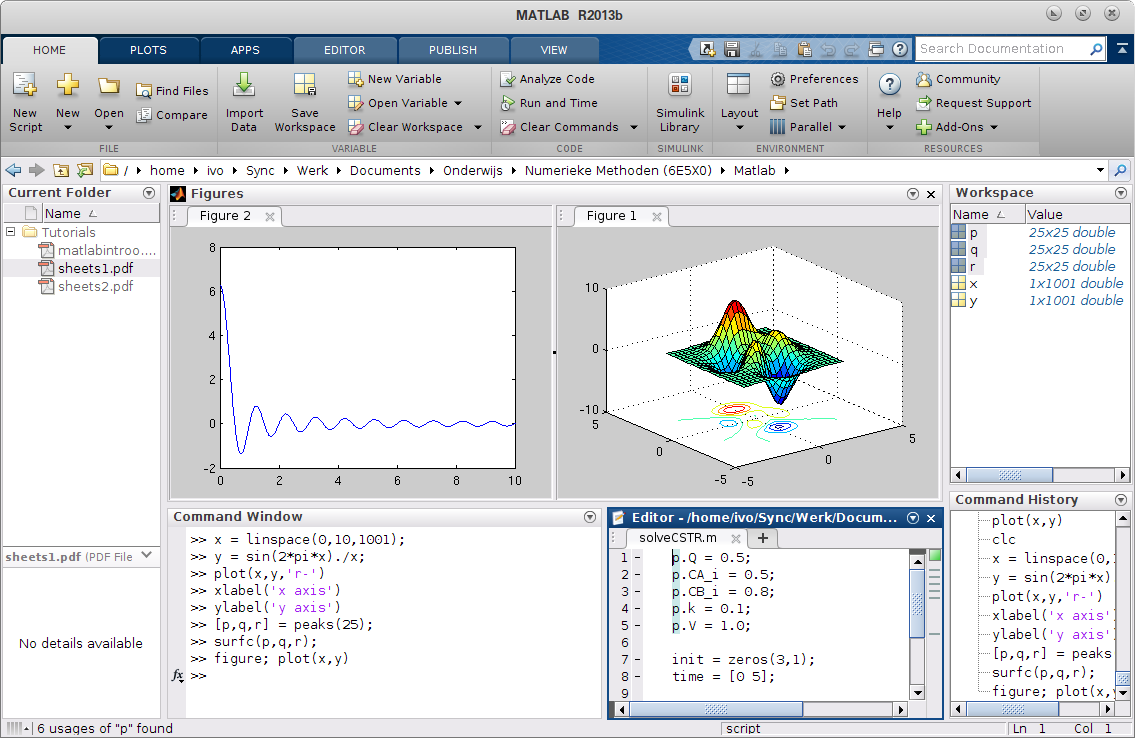
\includegraphics[width=0.7\textwidth]{matlab.png}
\end{frame}

\begin{frame}
\frametitle{Versatility of Matlab: ODE solver}
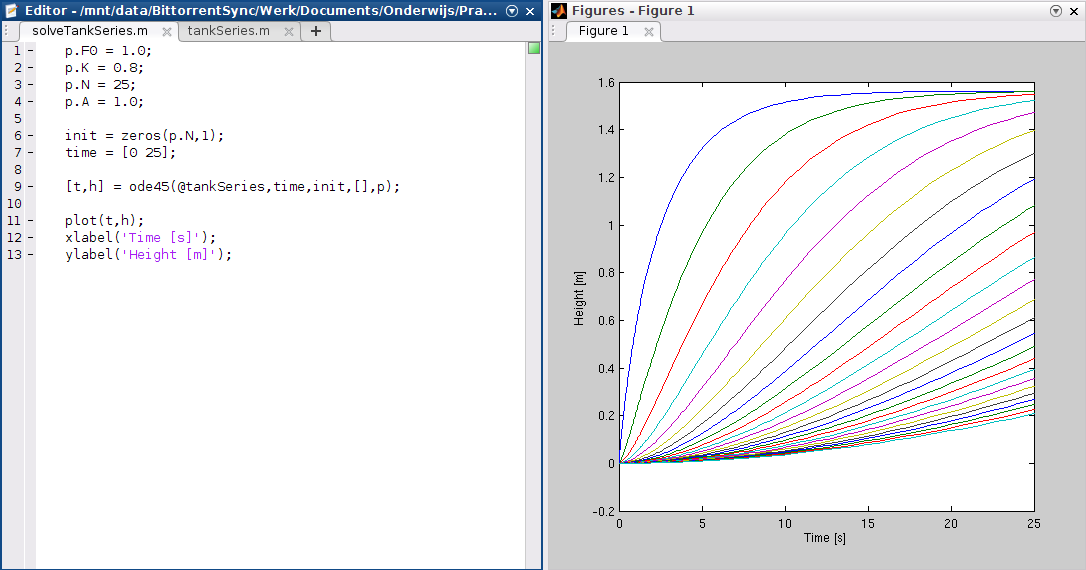
\includegraphics[width=\textwidth]{odesol.png}
\end{frame}

\begin{frame}[fragile]
\frametitle{Versatility of Matlab: Image analysis}
\begin{columns}
  \column{0.5\textwidth}
\begin{lstlisting}
I = imread('bubbles.png');
BW = rgb2gray(I);
E = edge(BW, 'canny');
F = imfill(E, 'holes');
result = regionprops(F);
\end{lstlisting}  
\column{0.5\textwidth}
  \vfill
  \includegraphics<1>[width=\columnwidth]{bub1.png}
  \includegraphics<2>[width=\columnwidth]{bub2.png}
  \includegraphics<3>[width=\columnwidth]{bub3.png}
  \includegraphics<4>[width=\columnwidth]{bub4.png}
\end{columns}
\end{frame}

\begin{frame}
\frametitle{Versatility of Matlab: Curve fitting}
\centering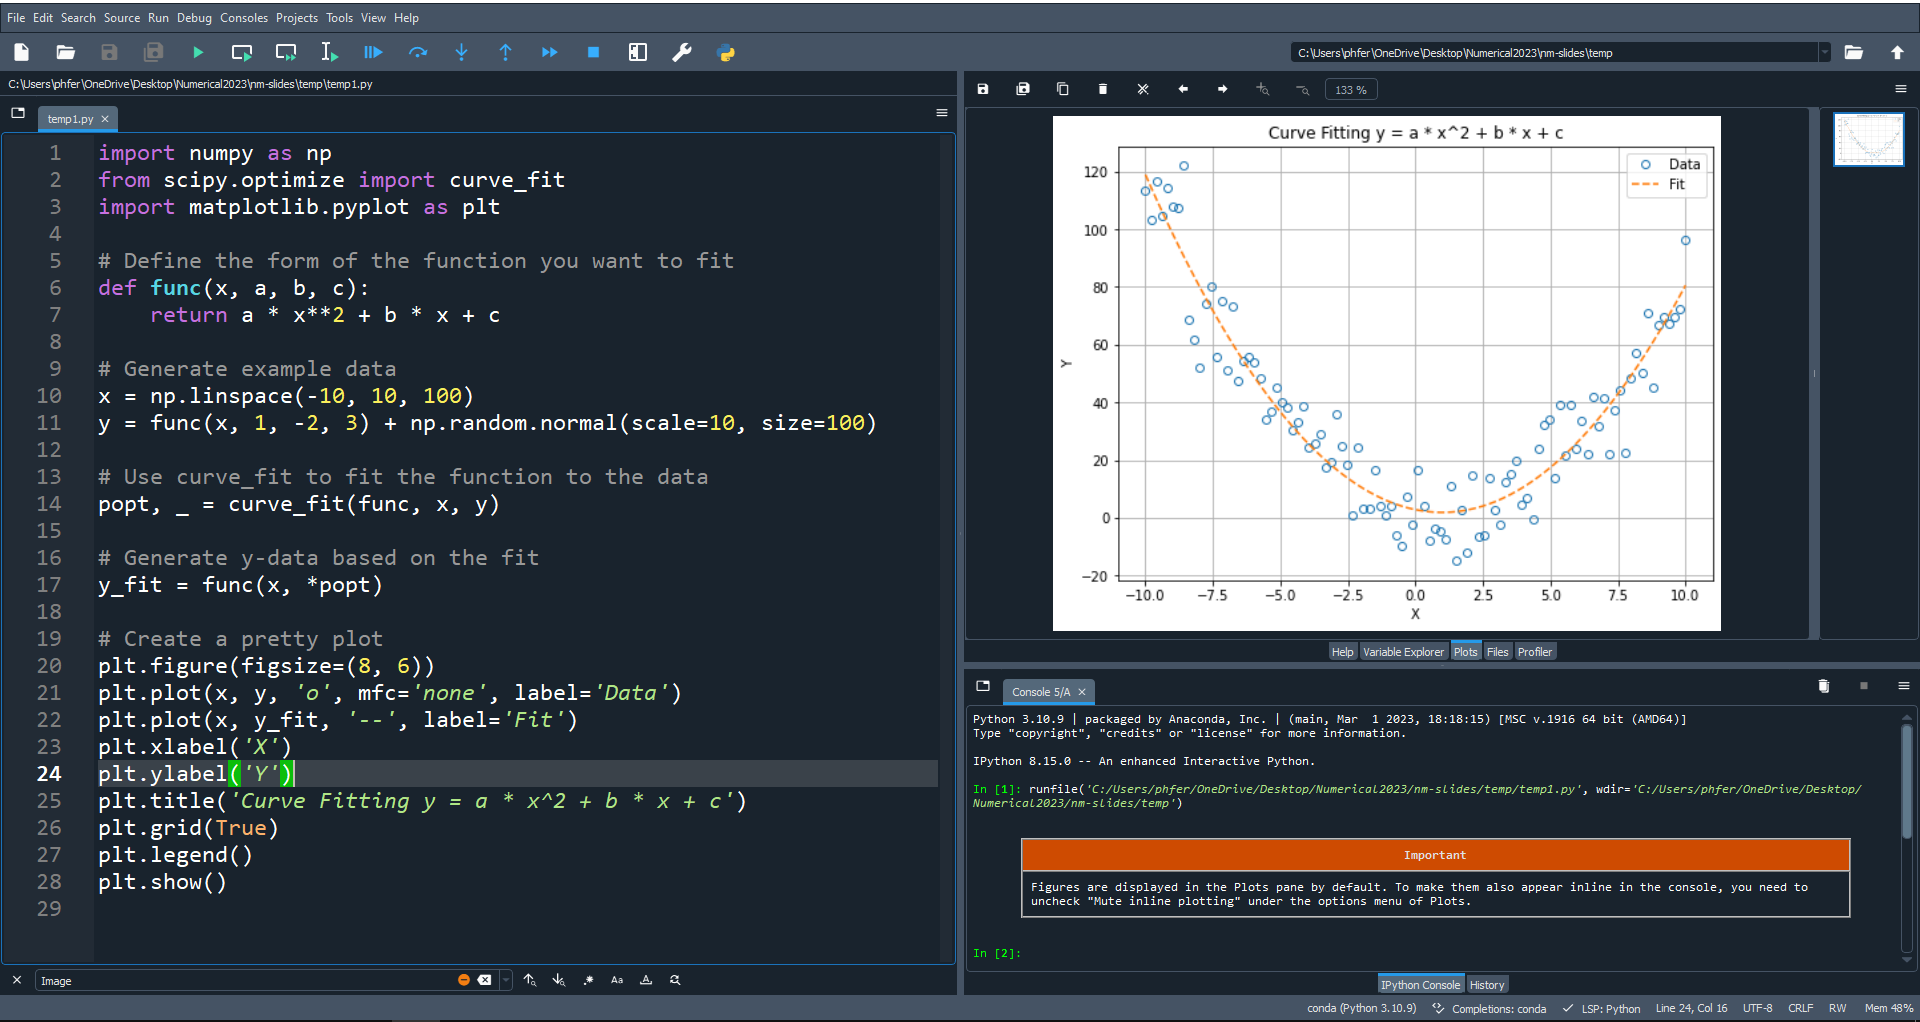
\includegraphics[width=0.7\textwidth]{cftool.png}
\end{frame}

\begin{frame}[fragile]
  \frametitle{Getting started}
   Start Matlab, and enter the following commands on the command line. Evaluate the output.
   \pause
   \begin{lstlisting}
 >> 2 + 3        % Some simple calculations
 >> 2*3
 >> 2*3^2        % Powers are done with ^ (*@ \pause @*)
 >> a = 2        % Storing values into the workspace
 >> b = 3
 >> c = (2*3)^2  % Parentheses set priority
 >> 8/a-b (*@ \pause @*)
 >> sin(a)       % Mathematical functions can be used 
 >> sin(0.5*pi)  % pi is an internal Matlab variable
 >> 1/0          % Infinity is a thing ...
 >> sqrt(-1)     % ... as are imaginary numbers
   \end{lstlisting}
 \end{frame}
 
 \begin{frame}[fragile]
   \frametitle{Printing and formatting results}
   You can control the display format of the output of a command using the \lstinline$format$ statement. This only involves the way the numbers are printed on the screen, behind the scenes the accuracy is the same (some 15 digits).
   \begin{lstlisting}
 >> format short % This is the default setting
 >> a = 19/4
 >> b = a^(-6)
 >> format long
 >> c = sqrt(21)
 >> d = exp(-c)
 >> format long e
 >> d = exp(-c)
 >> format short compact
 >> d
   \end{lstlisting}\pause
   A semi-colon at the end of a line suppresses output entirely:
   \begin{lstlisting}
 >> f = pi/4;
   \end{lstlisting}
 \end{frame}
 
 \begin{frame}[fragile]
  \frametitle{A few helpful things}
  \begin{itemize}[<+->]
    \item Using the \keystroke{$\uparrow$} and \keystroke{$\downarrow$} keys, you can cycle through recent commands
    \item Typing part of a command and pressing \keystroke{Tab} completes the command and lists the possibilities
    \item If a computation takes too long, you can press \keystroke{Ctrl}+\keystroke{C} to stop the program and return to the command line. Note that you may end up with incomplete results in the workspace.
    \item Sequences of commands (programs, scripts) are contained as m-files, plain text files with the \lstinline$.m$ extension.
    \item Such m-files must be in the \emph{current working directory} or in the Matlab \emph{path}, the locations where Matlab searches for a command. If you try to run a script that is not in the path, Matlab will suggest to add that directory to the \emph{path}, or to switch to that directory. Type \lstinline$path$ to view the current path.
    \item Anything following a \lstinline$%$ symbol is regarded as a comment
    \item In a script, pressing \keystroke{Ctrl}+\keystroke{R} comments the current line (or selection), \keystroke{Ctrl}+\keystroke{T} does the opposite.
    \item Clear the workspace by \lstinline$clear$, clear the command window by \lstinline$clc$.
  \end{itemize}
\end{frame}

\begin{frame}[fragile]
\frametitle{Matlab help, documentation, resources}
\begin{itemize}[<+->]
  \item You can look for a command with a particular purpose using the \lstinline$lookfor$ command:
  \begin{lstlisting}
>> lookfor inverse
  \end{lstlisting}
  \item Refer to the Matlab documentation using \lstinline$doc$ (pops up a new window) or \lstinline$help$ function
  \begin{itemize}
    \item Try for instance: \lstinline$help inv$ or \lstinline$help help$.
  \end{itemize}
  \item We supplied a number of basic Canvas modules: Matlab Crash Course, including small exercises.
  \item Matlab Academy: \url{https://matlabacademy.mathworks.com}
  \item Introduction to Numerical Methods and Matlab Programming for Engineers. T. Young and M.J. Mohlenkamp (2015). GNU-licensed document, online
  \item Search the web, Reddit, YouTube, etc.
\end{itemize}
\end{frame}

\section{Data structures}
\subsection*{Introduction}
\againframe<2>{contents_prog1}
\begin{frame}
 \frametitle{Terminology}
 \begin{description}
  \item[Variable] Piece of data stored in the computer memory, to be referenced and/or manipulated
  \item[Function] Piece of code that performs a certain operation/sequence of operations on given input
  \item[Operators] Mathematical operators (e.g. \lstinline$ + - *$ or \lstinline$/$), relational (e.g. \lstinline$< >$or \lstinline$==$, and logical operators (\lstinline$&&$, \lstinline$||$)
  \item[Script] Piece of code that performs a certain sequence of operations without specified input/output
  \item[Expression] A command that combines variables, functions, operators and/or values to produce a result.
 \end{description}
\end{frame}

\begin{frame}[fragile]
 \frametitle{Variables in Matlab}
  \begin{itemize}
   \item Matlab stores variables in the \emph{workspace}\pause
   \item You should recognize the difference between the \emph{identifier} of a variable (its name, e.g. \lstinline$x$, \lstinline$setpoint_p$), and the data that it actually stores (e.g. 0.5)\pause
   \item Matlab also defines a number of variables by default, e.g. \lstinline$eps$, \lstinline$pi$ or \lstinline$i$.\pause
   \item You can assign a variable by the \lstinline$=$ sign:
   \begin{lstlisting}
>> x = 4*3
x =
    12
   \end{lstlisting}\pause
   \item If you don't assign a variable, it will be stored in \lstinline$ans$
   \item Clearing the workspace is done with \lstinline$clear$.
 \end{itemize}
\end{frame}

\begin{frame}[fragile]
    \frametitle{Datatypes and variables}
    Matlab uses different types of variables:
        \begin{longtable}{l!{\vrule}l}
         Datatype        & Example \\ \hline
         \texttt{string} & \lstinline$'Wednesday'$ \\
         \texttt{integer}& \lstinline$15$ \\
         \texttt{float}  & \lstinline$0.15$ \\
         \texttt{vector} & \lstinline$[0.0; 0.1; 0.2]$ \\
         \texttt{matrix} & \lstinline$[0.0 0.1 0.2; 0.3 0.4 0.5]$ \\
         \texttt{struct} & \lstinline$sct.name = 'MyDataName'$ \\
                         & \lstinline$sct.number = 13$ \\
         \texttt{logical}& \lstinline$0$ (false)  \\
                         & \lstinline$1$ (true) \\
       \end{longtable}
   \end{frame}
   
   \begin{frame}[fragile]
    \frametitle{About variables}
    \begin{itemize}
      \item Matlab variables can change their type as the program proceeds (this is not common for other programming languages!):
      \begin{lstlisting}
   >> s = 'This is a string'
   s =
   This is a string
   >> s = 10
   s =
       10
   \end{lstlisting}
       \item Vectors and matrices are essentially \emph{arrays} of another data type. A vector of \lstinline$struct$ is therefore possible.
       \item Variables are \emph{local} to a function (more on this later).
   \end{itemize}
   \end{frame}

\subsection*{Vectors}
\begin{frame}[fragile]
  \frametitle{Vectors in Matlab (1)}
  A row vector:
  \begin{lstlisting}
>> v = [0 1 2 3]
  \end{lstlisting}\pause
  A column vector by separating elements with semi-colons:
  \begin{lstlisting}
>> u = [9; 10; 11; 12; 13; 14; 15]
  \end{lstlisting}\pause
  Access (i.e. read) an entry in a vector:
  \begin{lstlisting}
>> u(2)
  \end{lstlisting}\pause
  Manipulate the value of that entry:
  \begin{lstlisting}
>> u(2)=47
  \end{lstlisting}\pause
  Get a slice of a vector:
  \begin{lstlisting}
>> u([2 3 4]) % With colon operator: u(2:4)
  \end{lstlisting}\pause
  Transposing vectors:
  \begin{lstlisting}
>> w = v'
  \end{lstlisting}
\end{frame}

\begin{frame}[fragile]
  \frametitle{Vectors in Matlab (2)}
  Manual definition may be cumbersome. A colon (\lstinline$:$) generates a list:
  \begin{lstlisting}
>> a = 1:10      % Default stride is 1
>> x = -1:.1:1   % start:stride:stop specifies list
  \end{lstlisting}\pause
  Or, when you prefer to set the \emph{number of elements} instead of the step size:
  \begin{lstlisting}
>> y = linspace(0,10,11)
>> p = logspace(2,6,5)
  \end{lstlisting}\pause
  Manipulating multiple components:
  \begin{lstlisting}
>> y([1 4:7]) = 1
  \end{lstlisting}\pause
  Or (by supplying a vector instead of a scalar):
  \begin{lstlisting}
>> y([1 4:7]) = 16:20 % equivalent to y([1 4 5 6 7]) = [16 17 18 19 20]
  \end{lstlisting}
\end{frame}

\begin{frame}[fragile]
 \frametitle{Practice}
 Given a vector 
 \[ 
    x = \left[2 \ 4 \ 6 \ 8 \ 10 \ 12 \ 14 \ 16 \ 18 \ 20 \ 30 \ 40 \ 50 \ 60 \ 70 \ 80 \right]
 \]
 \begin{itemize}
  \item Find a way to define the vector without typing all individual elements\pause
  \item Investigate the meaning of the following commands:
  \begin{lstlisting}
>> x(3)
>> x(1:5)
>> x(1:end-1)
>> y = x(5:end)
>> y(4)
>> y(4) = []
>> sum(x)
>> mean(x)
>> std(x)
>> max(x)
>> fliplr(x)
>> x(end:-1:1)
>> diff(x)
  \end{lstlisting}
 \end{itemize}
\end{frame}

\begin{frame}[fragile]
  \frametitle{Practice}
  Given a vector 
  \[ 
     x = \left[2 \ 4 \ 6 \ 8 \ 10 \ 12 \ 14 \ 16 \ 18 \ 20 \ 30 \ 40 \ 50 \ 60 \ 70 \ 80 \right]
  \]
  \begin{itemize}
   \item Find a way to define the vector without typing all individual elements\pause
   \item Investigate the meaning of the following commands:
   \begin{lstlisting}
 >> y = x(5:end)
 >> y(4)
 >> y(4) = []
 >> sum(x)
 >> mean(x)
 >> std(x)
 >> max(x)
 >> fliplr(x)
 >> diff(x)
   \end{lstlisting}
  \end{itemize}
 \end{frame}

\begin{frame}[fragile]
  \frametitle{Operations on vectors (1)}
  \begin{lstlisting}
>> e = 1:5
>> f = 2*e
>> g = 4*f + 20 (*@ \pause @*)
>> h = e^2
  \end{lstlisting}\pause
  ... wait ... what's that?
  \begin{lstlisting}[basicstyle=\color{red}\footnotesize\ttfamily,keywordstyle={\color{red}}, identifierstyle=\color{red}]
Error using  ^ 
Inputs must be a scalar and a square matrix.
To compute elementwise POWER, use POWER (.^) instead.
  \end{lstlisting}\pause
  Matlab uses matrix operations by default, we should use a dot operator to make operations element-wise for \lstinline$*$, \lstinline$/$ and \lstinline$^$.
  \begin{lstlisting}
>> e.^2
  \end{lstlisting}
\end{frame}

\begin{frame}[fragile]
  \frametitle{Operations on vectors (2)}
   To demonstrate the matrix product:
  \begin{lstlisting}
>> p = [1; 1; 1]
>> q = [1 2 3]
>> p*q   % which is not equal to q*p
  \end{lstlisting}\pause
  All kinds of mathematical functions on vectors typically operate on elements:
  \begin{lstlisting}
    >> x = linspace(0,2*pi,100);
    >> s = sin(x)
    >> e = exp(x)
  \end{lstlisting}
\end{frame}

\subsection*{Matrices}
\begin{frame}[fragile]
  \frametitle{Matrices in Matlab}
  \begin{columns}[T]
   \column{0.35\textwidth}
    Matrix A is defined as:
    \[
    A = \begin{bmatrix}
      8 & 1 & 6 \\
      3 & 5 & 7 \\
      4 & 9 & 2
    \end{bmatrix}\]
    \pause
    \column{0.65\textwidth}
    In Matlab:
  \begin{lstlisting}
>> A = [ 8 1 6; 3 5 7; 4 9 2]
  \end{lstlisting}
  \end{columns}
  \pause
  Elements can be accessed/manipulated by the following syntax:
  \begin{lstlisting}
>> A(3,1) % Third row, first column, also A(3)
>> A(3,:) = [2 4 8] % Set entire third row
>> A(:,3) % Print third column
>> A(A>5) = 2 % Set elements by condition
  \end{lstlisting}\pause
  There are a few functions that help creating matrices:
  \begin{lstlisting}
>> A = zeros(4)  % A 4x4 matrix with zeros
>> A = ones(4,1) % A 4-element vector with ones
>> A = eye(3)    % Identity matrix of 3x3
>> A = rand(3,4) % A 3x4 matrix with random numbers
  \end{lstlisting}
\end{frame}

\begin{frame}[fragile]
 \frametitle{Practice}
 \begin{itemize}
  \item Find a \emph{short} Matlab expression to create the following matrix:
  \[
   A = \begin{bmatrix}
        1 & 2 & 3 & 4 & 5 & 6 & 7\\
        9 & 7 & 5 & 3 & 1 & -1 & -3 \\
        4 & 8 & 16 & 32 & 64 & 128 & 256 \\
       \end{bmatrix}
  \]\pause
  \item Investigate the command \lstinline$max(A)$. What does it give?
%   \item How to obtain the maximum for each row?
 \end{itemize}
\end{frame}

\begin{frame}
 \frametitle{Building blocks: Mathematics and number manipulation}
 Programming languages usually support the use of various mathematical functions (sometimes via a specialized library). Some examples of the most elementary functions in Matlab:
    \begin{longtable}{l!{\vrule}l}
      Command        & Explanation \\ \hline
      \texttt{cos(x), sin(x), tan(x)} & Cosine, sine or tangens of $x$ \\
      \texttt{mean(x), std(x)} & Mean, st. deviation of vector $x$ \\
      \texttt{exp(x)} & Value of the exponential function $e^x$ \\
      \texttt{log10(x), log(x)} & Base-10/Natural logarithm of $x$ \\
      \texttt{floor(x)} & Largest integer smaller than $x$ \\
      \texttt{ceil(x)} & Smallest integer that exceeds $x$ \\
      \texttt{abs(x)} & Absolute value of $x$ \\
      \texttt{size(x)} & Size of a vector $x$ \\
      \texttt{length(x)} & Number of elements in a vector $x$ \\
      \texttt{rem(x,y)} & Remainder of division of $x$ by $y$\\
    \end{longtable}
\end{frame}

\section{Plotting}
\subsection*{Simple plotting}
\againframe<2>{contents_prog1}
\begin{frame}[fragile]
  \frametitle{Simple plotting}
  Let's make a plot of the following table
   \begin{longtable}{l!{\vrule}ccccc}
%    \rowcolors[]{1}{maincolor!20}{maincolor!10}
      T ($^\circ$C) & 5   &  20  & 30   & 50   & 55 \\
      $\mu$ (Pa$\cdot$s)  & 0.08& 0.015& 0.009& 0.006& 0.0055 \\
    \end{longtable} \pause
  \begin{lstlisting}
>> T = [ 5 20 30 50 55 ]
>> mu = [ 0.08 0.015 0.009 0.006 0.0055]
\end{lstlisting}
\begin{onlyenv}<1-2>
  \begin{lstlisting}
>> plot(T,mu)
  \end{lstlisting}
\end{onlyenv}
\begin{onlyenv}<3>
  \begin{lstlisting}
>> plot(T,mu,'*')
  \end{lstlisting}
\end{onlyenv}
\begin{onlyenv}<4>
  \begin{lstlisting}
>> plot(T,mu,'r--')
  \end{lstlisting}
\end{onlyenv}
\begin{onlyenv}<5>
  \begin{lstlisting}
>> plot(T,mu,'ko-','LineWidth',2)
  \end{lstlisting}
\end{onlyenv}
\begin{lstlisting}
>> xlabel('Temperature [^\circC]')
>> ylabel('Viscosity [Pa s]')
>> title('Experiment 1')
  \end{lstlisting}
\end{frame}

\begin{frame}[fragile]
 \frametitle{Practice}
 Create plots of the following functions in a single figure for $x \in \left\{0,2\pi\right\}$:
  \[
    y_1 = \cos x 
  \]
  \[
    y_2 = \arctan x 
  \]
  \[
    y_3 = \frac{\sin x }{x}
  \]
  \pause
  Strategies to draw multiple graphs in 1 figure:
 \begin{lstlisting}
>> plot(x,y1,x,y2,x,y3)
 \end{lstlisting}
  \begin{lstlisting}
>> plot(x,y1)
>> hold on; % Maintain drawn plots in current figure
>> plot(x,y2)
>> plot(x,y3) % The 'hold-property' was already set
  \end{lstlisting}
\end{frame}

\begin{frame}[fragile]
  \frametitle{Multiple graph plotting}
  \begin{itemize}
    \item A new figure window can be created using the \lstinline$figure$ command. 
    \item The command \lstinline$subplot(m,n,p)$ divides the figure window into blocks using \lstinline$m$ rows and \lstinline$n$ columns. The number or vector \lstinline$p$ indicates which block (from left to right, top to bottom) or blocks are used for the axis.
    \item Graph operators (e.g. axis labels, title, hold on, etc) act on the active subplot
    \begin{lstlisting}
      x = linspace(0,2*pi,1000)
      y1 = sin(x);
      y2 = cos(x);
      y3 = tan(x);
      subplot(2,2,1); plot(x,y); title('sin(x)');
      subplot(2,2,1); plot(x,y1); title('sin(x)');
      subplot(2,2,3); plot(x,y2); title('cos(x)')
      subplot(2,2,[2 4]); plot(x,y3); title('tan(x)'); axis([0 2*pi -10 10])
    \end{lstlisting}
  \end{itemize}
\end{frame}

\begin{frame}[fragile]
  \frametitle{Multiple graph plotting}
  \begin{center}
    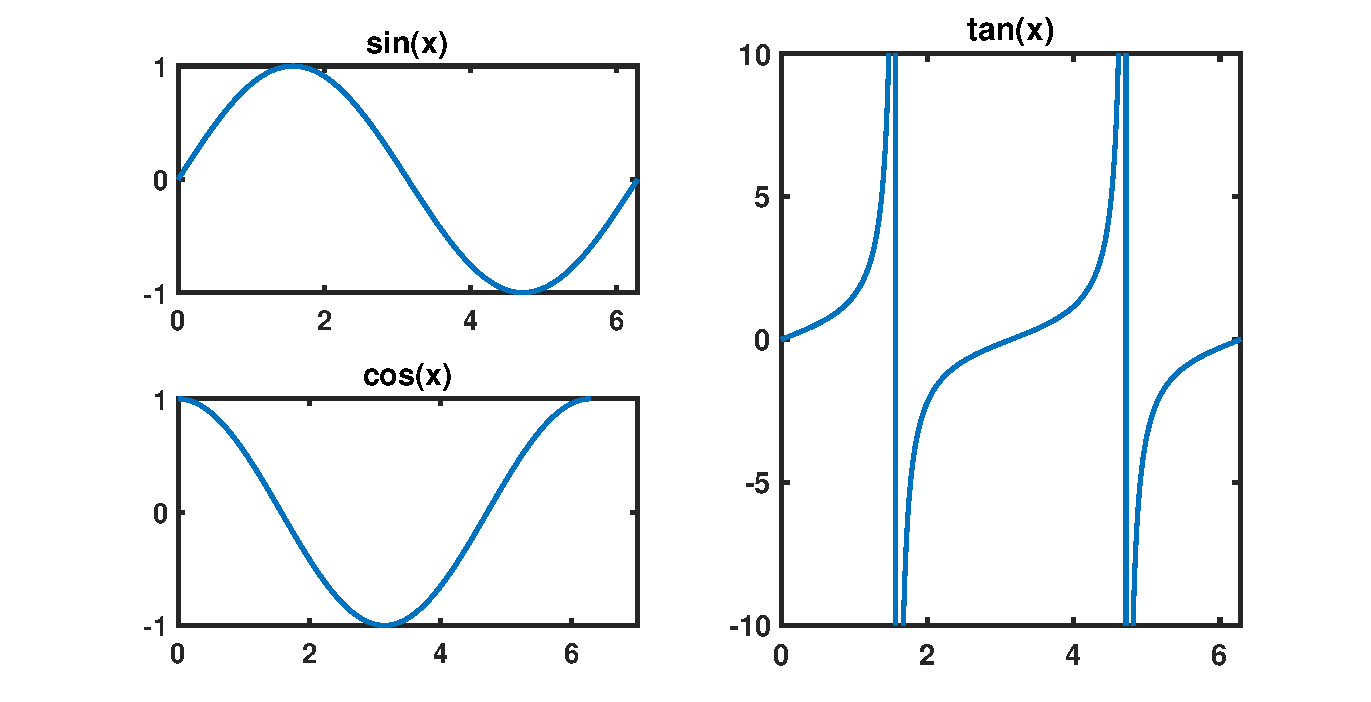
\includegraphics[width=0.8\textwidth]{subplot-demo}
  \end{center}

\end{frame}

\section{Creating algorithms}
\subsection*{Control statements}
\againframe<2>{contents_prog1}
\begin{frame}[fragile]
 \frametitle{Building blocks: conditional statements}
  \lstinline$if$-statement: Check whether a (set of) condition(s) is met, based on relational operations. \\ 
  \vskip1em \pause
  \begin{lstlisting}
num = floor (10 * rand + 1);
guess = input ('Your guess please : ');
if ( guess ~= num )
  disp (['Wrong, it was ',num2str(num),'. Kbye.']);
else
    disp ('Correct !') ;
end
  \end{lstlisting}
  \pause
  \begin{columns}[T]
    \column{0.5\textwidth}
    Other relational operators
      \begin{longtable}{l!{\vrule}l}
      \hline
      \lstinline$==$& is equal to \\ 
      \lstinline$~=$& is not equal to \\ 
      \lstinline$<=$& is less than or equal to\\
      \lstinline$>=$&is  greater than or equal to\\
      \lstinline$<$& is less than \\
      \lstinline$>$& is greater than \\
      \hline
    \end{longtable}  
    \column{0.5\textwidth}
      Combining conditional statements
      \begin{longtable}{l!{\vrule}l}
      \hline
      \lstinline$&$& and \\ 
      \lstinline$|$& or\\
      \lstinline$~$& negation (switches true/false)\\
      \lstinline$xor$& exclusive or\\
      \hline
    \end{longtable}  
  \end{columns}
\end{frame}

\begin{frame}[fragile]
 \frametitle{Building blocks: conditional statements}
  You can use nested \lstinline$if$-statements and combinations of expressions:
  \begin{lstlisting}
a = 3;
b = 9;

if (a < b) & (b <= 10)
    disp('a is smaller than 10 (by deduction)')
elseif ((a >= b) & (b > 10))
        disp('a is larger than 10 (by deduction)')
else
    disp('We cannot deduce if a is smaller than 10 or not, unless we perform a direct comparison')
    if (a < 10)
        disp('a is smaller than 10')
    elseif (a > 10)
        disp('a is larger than 10')
    else 
        disp('a is equal to 10')
    end
end
\end{lstlisting}
\end{frame}

\begin{frame}[fragile]
  \frametitle{Building blocks: logical indexing}
   Relational operators return a type "logical", i.e. true (1) or false (0). You can use this to select subsets of existing vectors. 
   \vskip2em
   \begin{columns}
    \column{0.5\textwidth} 
    Simple demonstration:
    \begin{lstlisting}
>> x = linspace(-3,3,7) % Create a base vector
x =
    -3    -2    -1     0     1     2     3
>> x>0 % Illustrate logical result
ans =
  1x7 logical array
   0   0   0   0   1   1   1
>> x2 = x(x>0) % Create a subset
x2 =
     1     2     3
    \end{lstlisting}\pause
    \column{0.5\textwidth} 
    You can use the same logical index for different vectors (in script-format):
    \begin{lstlisting}
% Create a base vector
x  = linspace(-4*pi,4*pi,1000);
y = (sin(x)+0.2*x)+1;
% Select only values where y>0 and plot
xs = x(y>0); ys = y(y>0);
plot(x,y,xs,ys)
    \end{lstlisting}
  \end{columns}
 \end{frame}

 \begin{frame}[fragile]
  \frametitle{Practice relational operations and logical indexing}
  \begin{enumerate}
    \item Let \lstinline$x = [1 5 2 8 9 0 1]$ and \lstinline$y = [5 2 2 6 0 0 2]$. Execute and explain the results of the following commands:
    \begin{columns}
      % \column{0.05\textwidth}
      \column{0.25\textwidth}
        \begin{itemize}
          \item \lstinline$x > y$
          \item \lstinline$y < x$
          \item \lstinline$x == y$
        \end{itemize}
      \column{0.25\textwidth}
        \begin{itemize}
          \item \lstinline$x <= y$
          \item \lstinline$y >= x$
          \item \lstinline$x | y$
        \end{itemize}
      \column{0.25\textwidth}
        \begin{itemize}
          \item \lstinline$x & (~y)$
          \item \lstinline$(x > y) | (y < x)$
          \item \lstinline$(x > y) & (y < x)$
        \end{itemize}
    \end{columns}
    \vskip1em
  \item Clear the workspace. Let \lstinline$x = 1:10$ and \lstinline$y = [3 5 6 1 8 2 9 4 0 7]$. The exercises here show the techniques of logical-indexing. Execute and interpret the results of the following commands:
    \begin{itemize}
      \item \lstinline$(x > 3) & (x < 8)$
      \item  \lstinline$x(x > 5)$
      \item  \lstinline$y(x <= 4)$
      \item  \lstinline$x((x < 2)|(x>=8))$
      \item  \lstinline$y((x < 2)|(x>=8))$
      \item  \lstinline$x(y<0)$
    \end{itemize}
  \end{enumerate}
 \end{frame}

\begin{frame}[fragile]
 \frametitle{Building blocks: case selection}
  \lstinline$switch$-statement: Selects and runs a block of code. \\ 
  \vskip1em \pause
  \begin{lstlisting}
[dnum,dnam] = weekday(now);
switch dnum
    case {1,7}
        disp('Yay! It is weekend!');
    case 6
        disp('Hooray! It is Friday!');
    case {2,3,4,5}
        disp(['Today is ' dnam]);
    otherwise
        disp('Today is not a good day...');
end
  \end{lstlisting}
\end{frame}
    
\begin{frame}[fragile]
 \frametitle{Building blocks: loops}
  \lstinline$for$-loop: Performs a block of code a certain number of times. \\ 
  \vskip1em \pause
  \begin{lstlisting}
>> p(1) = 1;
>> p(2) = 1;
>> for i = 2:10
p(i+1) = p(i)+p(i-1);
end
>> p
p =
   1   1   2   3   5   8  13  21  34  55  89
  \end{lstlisting}
\end{frame}

\begin{frame}[fragile]
 \frametitle{Building blocks: indeterminate repetition}
  \lstinline$while$-loop: Performs and repeats a block of code until a certain condition. \\ 
  \vskip1em \pause
  \begin{lstlisting}
num = floor (10* rand +1) ;
guess = input ('Your guess please : ');

while ( guess ~= num )
    guess = input ('That is wrong. Try again ... ');
end

if (isempty(guess))
    disp('No number supplied - exit');
else
    disp ('Correct!');
end
  \end{lstlisting}
\end{frame}

%%%% Example
\begin{frame}[fragile]
 \frametitle{Example algorithm}
 Compute the factorial of $N$: $N! = N\cdot(N-1)\cdot(N-2)\cdots 2\cdot 1$\\ \vskip1em
 How to deal with this? \vfill
 \begin{columns}[T]
  \column{0.3\textwidth}
  \begin{block}<2->{Naive approach}
      \begin{lstlisting}
Z = 1;
Z = Z*2;
Z = Z*3;
Z = Z*4;
... etc ...      
      \end{lstlisting}
  \end{block}
  \column{0.3\textwidth}
  \begin{block}<3->{For-loop}
      \begin{lstlisting}
Z = 1;
for i = 1:N
    Z = Z*i;
end
      \end{lstlisting}
  \end{block}
  \column{0.3\textwidth}
\begin{block}<4>{While-loop}
      \begin{lstlisting}
Z = 1;
i = 1;
while (i<=N)
    Z = Z*i;
    i = i+1;
end
      \end{lstlisting}
  \end{block}
 \end{columns}
 \onslide<4>{
  Note: \lstinline$N$ must be set beforehand!\\ 
  Note: Pay attention to the relational operators!  }
\end{frame}

\begin{frame}[fragile]
 \frametitle{Input and output}
 Many programs require some input (data) to function correctly. A combination of the following is common:
 \begin{itemize}[<+->]
   \item Input may be given in a parameters file (``hard-coded'')
   \item Input may be entered via the keyboard
   \begin{lstlisting}
    >> a = input('Please enter the number ');
  \end{lstlisting}
  \item Input may be read from a file, e.g.
  \begin{lstlisting}
    >> data = getfield(importdata('myData.txt', ' ', 4), 'data');
    >> numdata = xlsread('myExcelDataFile.xls');
  \end{lstlisting}
  Importdata also has a GUI equivalent (right-click on file, select \emph{Import Data})
   \item There are many more advanced functions, e.g. \lstinline$fread$, \lstinline$fgets$, ...
 \end{itemize}
\end{frame}

\begin{frame}[fragile]
 \frametitle{Input and output}
 Output of results to screen, storing arrays to a file or exporting a graphic are the most common ways of getting data out of Matlab:
 \begin{itemize}[<+->]
   \item Results of each expression are automatically shown on screen as long as the line is not ended with a semi-colon;
   \item Output may be stored via the GUI:
    \begin{itemize}
      \item Use the 'Export Setup' function
      \item Save figure (use .fig, .eps or .png, \textbf{not} .jpg or .pcx)
      \item Save variables (right click, save as)
    \end{itemize}
   \item Save variables automatically (scripted):
    \begin{lstlisting}
>> savefile = 'test.mat';
>> p = rand(1,10);
>> q = ones(10);
>> save(savefile,'p','q')
   \end{lstlisting}
   \item More advanced functions can be found in e.g.  \lstinline$fwrite$, \lstinline$fprintf$, ...
 \end{itemize}
\end{frame}

\section{Functions}
\subsection*{Introduction}
\againframe<2>{contents_prog1}
\begin{frame}[fragile]
 \frametitle{Functions - general}
 A function in a programming language is a program fragment that performs a certain task. Creating functions keeps your code clean, re-usable and structured.
 \begin{itemize}
   \colorize<2> \item You can use functions supplied by the programming language, and define functions yourself
   \colorize<3> \item Functions take one or more input parameters (\emph{arguments}), and \emph{return} an output (result).
  %  \begin{itemize}
  %    \colorize<3-> \item If functions do not return a result, it is called a procedure
  %  \end{itemize}
   \colorize<4> \item In Matlab, functions are defined as follows (2 output and 3 input arguments):
  \begin{overlayarea}{\textwidth}{2em}
   \begin{onlyenv}<4->
    \begin{lstlisting}
function [out1, out2] = myFunction(in1, in2, in3)
    \end{lstlisting}
    \end{onlyenv}
   \end{overlayarea} 
   \item\colorize<5> In the function body, you can perform operations on the input parameters (\lstinline$in1$, \lstinline$in2$ and \lstinline$in3$. 
   \item\colorize<6> Inside a function, other values are not available (local workspace). Analogously, any variables created are not available after the function returns, except for those explicitly defined as output arguments.
   \item\colorize<7> The name of the function and the name of the file should be identical and (just like variables) be unique.
  \end{itemize}
\end{frame}

\begin{frame}[fragile]
  \frametitle{Functions - Exercise}
  Example: write a function that takes 3 variables, and returns the average: \pause
   \begin{columns}[T]
    \column{0.5\textwidth}
    \begin{block}<2->{Approach 1}
  \begin{lstlisting}
 function res = avg1(a,b,c)
     mySum = a + b + c;
     res = mySum / 3;
 end \end{lstlisting}
    \end{block}
    \column{0.5\textwidth}
    \begin{block}<3->{Approach 2}
        \begin{lstlisting}
 function res = avg2(a,b,c)
     data = [a; b; c];
     res = mean(data);
 end \end{lstlisting}
    \end{block}
  \end{columns}
 \end{frame}

\begin{frame}[fragile]
  \frametitle{Functions - definition overview}
  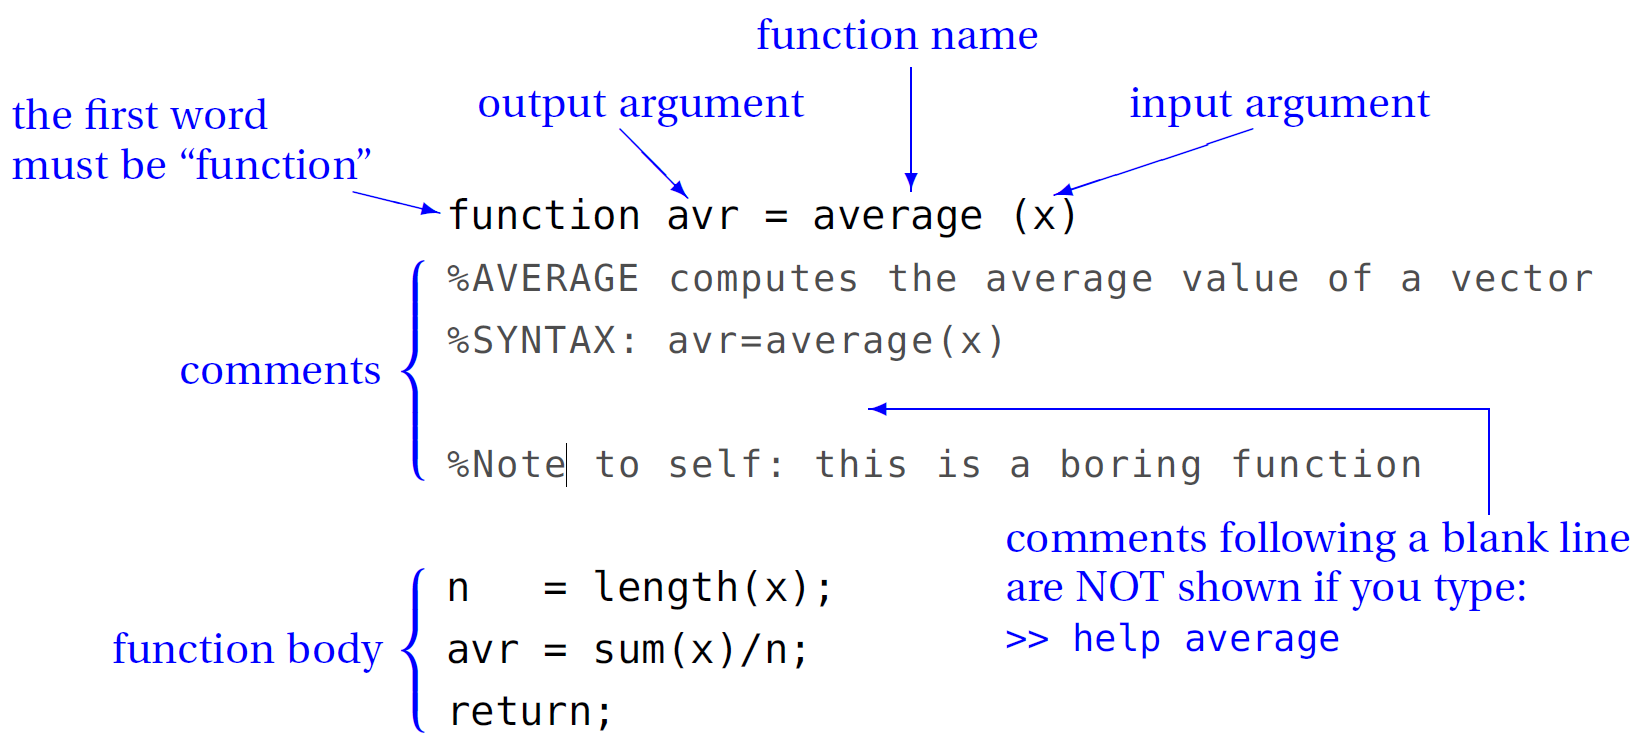
\includegraphics[width=\textwidth]{format-func.png}\footnote{Source: Pekalska, Meinsma and Zwart, Programming with Matlab manual, University of Twente, 2018.}
 \end{frame}

% \begin{frame}[fragile]
%  \frametitle{Functions - locality and arguments}
%  \begin{itemize}
%    \item You are supplying arguments to a function because it does not have acces to previously defined variables. This is called \emph{locality}.
%    \begin{itemize}
%      \item This does not include global variables - but they're evil!
%      \item Local variables created in a function are not accessible to other functions unless they are returned or supplied as an argument!
%    \end{itemize}
%  \end{itemize}
% \end{frame}

\begin{frame}[fragile]
 \frametitle{Functions - stack}
 Calling functions from each other creates a 'stack', like a stack of cards. The stack works with first in, last out (FILO) principle.
 \begin{columns}
 \column{0.5\textwidth}
    \begin{lstlisting}
function [] = a()
disp('Start of a()');
b();
disp('End of a()');
end

function [] = b()
disp('Start of b()');
c();
disp('End of b()');
end

function [] = c()
disp('Start of c()');
disp('End of c()');
end
    \end{lstlisting}
    \column{0.5\textwidth}
    \begin{lstlisting}
>> stackcheck
Start of a()
Start of b()
Start of c()
End of c()
End of b()
End of a()
    \end{lstlisting}
 \end{columns}
\end{frame}

\begin{frame}[fragile]
 \frametitle{Exercise: create a function}
 Compute $N! = N\cdot(N-1)\cdot(N-2)\cdots 2\cdot 1$\\ \vskip1em
 Create a function of our while-loop approach with N the argument: \\
 
 \begin{columns}[T]
   \column{0.5\textwidth}
   \begin{block}{Original script}
	   \begin{lstlisting}
Z = 1;
i = 1;
while (i<=N)
    Z = Z*i;
    i = i+1;
end \end{lstlisting}
   \end{block}
   \column{0.5\textwidth}
   \begin{block}<2>{Function}
	   \begin{lstlisting}
function Z = fact_while(N)

Z = 1;
i = 1;
while (i<=N)
    Z = Z*i;
    i = i+1;
end

end\end{lstlisting}
   \end{block}
 \end{columns}
\end{frame}

\begin{frame}[fragile]
 \frametitle{Functions - checking input}
  The function we created computes the factorial correctly! \pause
  \begin{itemize}
     \item When the supplied argument is positive\pause\ and \pause
     \item When the supplied argument is a natural number...
  \end{itemize}\pause
  \begin{columns}[T]
   \column{0.4\textwidth}
     
\includegraphics[width=\columnwidth]{deadmau5.png}
   \column{0.6\textwidth}
    \pause
    \begin{itemize}[<+->]
     \item In this case, we should check the user input to prevent an infinite loop: \pause
     \begin{lstlisting} 
if (fix(N)~=N) | (N<0)
    disp 'Provide a positive integer number!'
    return;
end \end{lstlisting}
      \item If no check can be done before a while-loop, you may want to stop after $x$ loops
    \end{itemize}
  \end{columns}
\end{frame}

\begin{frame}[fragile]
 \frametitle{Functions - checking input}
  The whole factorial function, including comments:
     \begin{lstlisting}
function Z = fact_while(N)
%% This function computes a factorial of input value N
% Usage  : fact_while(N)
% N      : value of which the factorial is computed
% returns: factorial of N

% Catch non-integer case
if (fix(N)~=N) | (N<0)
    disp 'Provide a positive integer number!'
    return;
end

Z = 1;
i = 1;
while (i<=N)
    Z = Z*i;
    i = i+1;
end

end \end{lstlisting}
\end{frame}

\begin{frame}[label=recursion,fragile]
 \frametitle{Recursion}
 \begin{columns}
   \column{0.5\textwidth}
   \begin{itemize}
    \item<1-> In order to understand recursion, one must first understand recursion
    \item<2-> A recursive function includes a call to itself (a function within a function)
    \begin{itemize}
      \item<3-> This could lead to infinite calls;
      \item<3-> A base case is required so that recursion is stopped;
      \item<3-> Base case does not call itself, simply returns.
    \end{itemize}
 \end{itemize}
   \column{0.5\textwidth}
   \includegraphics<3>[width=0.7\columnwidth]{scoobydoo.jpg}
 \end{columns}
\end{frame}

% \againframe{recursion}

\begin{frame}[fragile]
 \frametitle{Recursion: example}
 \begin{lstlisting}
function out = mystery(a,b)
if (b == 1)
    % Base case
    out = a;
else 
    % Recursive function call
    out = a + mystery(a,b-1);
end
 \end{lstlisting}
\vskip1em \pause
\begin{itemize}
  \item What does this function do? \pause
  \item Can you spot the error? \pause
  \item How deep can you go? Which values of b don't work anymore?
\end{itemize}
\end{frame}

\begin{frame}[fragile]
 \frametitle{Recursion: exercise}
 Create a function computing the factorial of $N$, based on recursion. \pause
 \begin{lstlisting}
function res = fact_recursive(x)

% Catch non-integer case
if (fix(x)~=x) | (x<0)
    disp 'You should provide a positive integer number only'
    return;
end

if (x > 1)
    res = x*fact_recursive(x-1);
else
    res = 1;
end

end 
 \end{lstlisting}
\end{frame}

\section{Conclusions}
\subsection*{Conclusions}
\againframe<2>{contents_prog1}
\begin{frame}[fragile]
  \frametitle{In conclusion...}
  \begin{itemize}
    \colorize<1> \item Matlab: A versatile development environment, with excellent vector and matrix computations
    \colorize<2> \item Programming basics: variables, operators and functions, locality of variables, recursive operations
  \end{itemize}
  \pause
    \begin{itemize}
    \colorize<3> \item For now: exercises on slide deck and Matlab modules
    \colorize<4> \item Preparation for next lecture: familiarize with the concepts, use Canvas course or Matlab Academy.
  \end{itemize}
\end{frame}

\section{Exercises}
\subsection*{Exercise 1}
\begin{frame}[fragile]
  \frametitle{Practice vectors and matrices}
  \begin{enumerate}
    \item Create a vector \lstinline$x$ with the elements:
    \begin{itemize}
      \item $[2,4,6,8,\ldots,16]$
      \item $[0, \frac{1}{2}, \frac{2}{3}, \frac{3}{4}, \ldots, \frac{99}{100}]$
    \end{itemize}
    \item Create a vector \lstinline$x$ with the elements: $x_n = \frac{(-1)^n}{2n-1}$ for $n=1,2,3,\ldots,200$. Find the sum of the first 50 elements $x_1,\ldots,x_{50}$.
    \item Let \lstinline$x = 20:10:200$. Create a vector \lstinline$y$ of the same length as \lstinline$x$ such that:
    \begin{itemize}
      \item $y_i = x_i - 3$
      \item $y_i = x_i$ for every even index $i$ and $y_i = x_i + 11$ for every odd index $i$.
    \end{itemize}
    \item Let \lstinline$T = [3 4; 1 8; -4 3]$ and \lstinline$ A = [diag(-1:2:3),T; -4 4 1 2 1]$. Perform
    the following operations on A:
    \begin{itemize}
      \item Retrieve a vector consisting of the 2nd and 4th elements of the 3rd row.
      \item Find the minimum of the 3rd column.
      \item Find the maximum of the 2nd row.
      \item Compute the sum of the 2nd column
      \item Compute the mean of the row 1 and the mean of row 4
    \end{itemize}
  \end{enumerate}
 \end{frame}

 \begin{frame}[fragile]
  \frametitle{Practice plotting}
  \begin{enumerate}
    \item Plot the functions $f(x)=x,\ g(x)=x^3,\ h(x)=e^x$ and $z(x)=e^{x^2}$ over the interval $[0,4]$ on the normal scale and on the log-log scale. Use an appropriate sampling to get smooth curves. Describe your plots by using the functions: \lstinline$xlabel$, \lstinline$ylabel$, \lstinline$title$ and \lstinline$legend$.
    \vskip1em
    \item Make a plot of the functions: $f(x)=sin(1/x)$ and $g(x)=cos(1/x)$ over the interval $[0.01,0.1]$. How do you create \lstinline$x$ so that the plots look sufficiently smooth?
  \end{enumerate}
 \end{frame}

 \begin{frame}[fragile]
  \frametitle{Practice control flow and loops (1)}
  \begin{enumerate}
    \item Write a function that uses two logical input arguments with the following behaviour:
    \begin{align*}
       f(\text{true},\text{true}) \mapsto \text{false} \\
      f(\text{false},\text{true}) \mapsto \text{true} \\ 
      f(\text{true},\text{false}) \mapsto \text{true} \\
      f(\text{false},\text{false}) \mapsto \text{false} \\
    \end{align*}
    \item Write a function that computes the factorial of x:
    \[ f(x) = x! = 1 \times 2 \times 3 \times 4 \times \ldots \times x \]
    \begin{itemize}
      \item Using a loop-construction
      \item Using recursion
    \end{itemize}
  \end{enumerate}
 \end{frame}

 \begin{frame}[fragile]
  \frametitle{Practice control flow and loops (2)}
  \begin{enumerate}
    \item Write a function that computes the exponential function using the Taylor series
    \[  e^x = 1 + x + \frac{x^2}{2!} + \frac{x^3}{3!} + \ldots \]
    until the last term is smaller than $10^{-6}$.
    \item Use a script to compute the result of the following series:
    \[
      f_n = \sum_{n=1}^{\infty} \frac{1}{\pi^2 n^2}
    \]
    This should give you an indication of the fraction this series converges to.
    \begin{itemize}
      \item Now plot in two vertically aligned subplots i) The result as a function of $n$, and ii) the difference with the earlier mentioned fraction as a function of n. For the latter, consider carefully the axis scale!
      % \item Use \lstinline$tic$ and \lstinline$toc$ to compare the computing times with $\pi^2$ inside vs outside the loop.
    \end{itemize}
  \end{enumerate}
 \end{frame}

 \begin{frame}[fragile]
  \frametitle{Practice logical indexing}
  \begin{enumerate}
    \item Let \lstinline$x = linspace(-4,4,1000)$, $y_1 = 3x^2 - 4x - 6$ and $y_2 = 1.5x - 1$. Use logical indexing to determine function $y_3 = \mathrm{max}(\mathrm{max}(y_1,y_2),0)$. Plot the function.
    \item Consider these data concerning the age (in years), length (in cm) and weight (in kg) of twelve adult men: \lstinline$A = [41 25 33 29 64 34 47 38 49 32 26 26]; H = [165 186 177 190 156 174 164 205 184 190 165 171]; W = [75 90 97 60 74 65 101 85 91 75 87 70];$.
    \begin{itemize}
      \item Calculate the average of all vectors (age, weight and length).
      \item Combine the command \lstinline$length$ with logical indexing to determine how many men in the group are taller than 182 cm.
      \item What is the average age of men with a body-mass index ($B \equiv \frac{W}{L^2}$ with $W$ in kg and $L$ in m) larger than 25? And for men with a $B<25$?
      \item How many men are older than the average and at the same time have a BMI below 25?
    \end{itemize}
  \end{enumerate}
 \end{frame}

\begin{frame}[fragile]
  \frametitle{Practice algorithm: Fourier series for heat equation}
  The unsteady 1D heat equation in 1D in a slab of material is given as:
  \[
     \frac{\partial T}{\partial t} = k\frac{\partial^2 T}{\partial x^2}
  \]
 We can express the temperature profile $T(x,t)$ in the slab using a Fourier sine series. For an initial profile T(x,0) = 20 and fixed boundary values T(0,t) = T(L,t) = 0, the solution is given as:
  \[
     T(x,t) = \sum_{n=1}^{n=\infty}\frac{40(1-(-1)^n)}{n\pi}  \sin\left(\frac{n\pi x}{L}\right) \exp\left(-kt\frac{n \pi}{L}^2\right)
  \]
  \begin{itemize}
      \item Create a script to solve this equation using loops and/or conditional statements
  \end{itemize}
 \end{frame}
 
%  \begin{frame}[fragile]
%   \frametitle{Fourier series for heat equation (1)}
%   A simple construct with a double loop.
%    \begin{lstlisting}
%  L = 2;
%  k = 0.004;
%  t = 3;
%  x = 0:0.1:L;
%  s = 0;
 
%  for n = 1:50
%      for i = 1:length(x)
%          pt(i) = 40*(1-(-1)^n)/(n*pi) * sin(n*pi*x(i)/L) * exp(-k*t*(n*pi/L)^2);
%      end
%      s = s + pt;
%  end
 
%  plot(x,s)
%    \end{lstlisting}
%  \end{frame}
 
%  \begin{frame}[fragile]
%   \frametitle{Fourier series for heat equation (2-1)}
%  We can also solve the equation for the entire x-range in 1 go. \lstinline$part$ and $s$ are both vectors. This is more efficient.
%    \begin{lstlisting}
%  L =  2;
%  x = linspace(0,L,101);
%  k = 0.004;
%  t = 3;
 
%  s = 0;
%  for n = 1:50
%      part = 40*(1-(-1)^n)/(n*pi) * sin(n*pi*x/L) * exp(-k*t*(n*pi/L)^2);
%      s = s + part;
%  end
 
%  plot(x,s)
%    \end{lstlisting}
%  \end{frame}
 
%  \begin{frame}[fragile]
%   \frametitle{Fourier series for heat equation (2-2)}
%  We can break the for-loop when the calculations are precise enough using an if-statement and a break-command.
%    \begin{lstlisting}
%  L = 2;
%  x = linspace(0,L,101);
%  k = 0.004;
%  t = 3;
 
%  s = 0;
%  for n = 1:2:50
%      part = 40*(1-(-1)^n)/(n*pi) * sin(n*pi*x/L) * exp(-k*t*(n*pi/L)^2);
%      s = s + part;
%      if (max(abs(part)) < 1e-6)
%          n
%          break
%      end
%  end
 
%  plot(x,s)
%    \end{lstlisting}
%  \end{frame}
 
%  \begin{frame}[fragile]
%   \frametitle{Fourier series for heat equation (3-1)}
%  We can run a while-loop for indeterminate iterations to ensure a certain precision while keeping computational demands to a minimum:
%    \begin{lstlisting}
%  L =  2;
%  x = linspace(0,2,101);
%  k = 0.004;
%  t = 3;
 
%  s = 0;
%  n = 1;
%  part = 1;
%  while (max(abs(part))>1e-6)
%      part = 40*(1-(-1)^n)/(n*pi) * sin(n*pi*x/L) * exp(-k*t*(n*pi/L)^2)
%      s = s + part;
%      n = n + 2;
%  end
 
%  n
%  plot(x,s)
%    \end{lstlisting}
%  \end{frame}
 
%  \begin{frame}[fragile]
%   \frametitle{Fourier series for heat equation (3-2)}
%  The \lstinline$drawnow$ command makes sure a plot is drawn before subsequent commands are executed. This gives us insight in the iteration process:
%    \begin{lstlisting}
%  L =  2;
%  x = linspace(0,2,101);
%  k = 0.004;
%  t = 3;
 
%  s = 0;
%  n = 1;
%  part = 1;
%  while (max(abs(part))>1e-6)
%      part = 40*(1-(-1)^n)/(n*pi) * sin(n*pi*x/L) * exp(-k*t*(n*pi/L)^2)
%      s = s + part;
%      n = n + 2;
%      plot(x,s)
%      pause(0.4)
%      drawnow
%  end
 
%  n
%    \end{lstlisting}
%  \end{frame}

%  \begin{frame}[fragile]
%   \frametitle{Fourier series for heat equation (as a function)}
%  A rudimentary function (i.e. no comments or checks) to get the heat equation profile for a given length, heat diffusivity and time:
%    \begin{lstlisting}
%  function [s,x] = fourier_series_heat_eqn(L,k,t)
%  x = linspace(0,L,101);
 
%  s = 0;
%  n = 1;
%  part = 1;
%  while (max(abs(part))>1e-6)
%      part = 40*(1-(-1)^n)/(n*pi) * sin(n*pi*x/L) * exp(-k*t*(n*pi/L)^2);
%      s = s + part;
%      n = n + 2;
%  end
%    \end{lstlisting}
   
%  Calling the function from a different script multiple times to plot a transient profile:
%  \begin{lstlisting}
%  for t = 0.01:0.01:30
%      [solution,xvec] = fourier_series_heat_eqn(2,0.004,t);
%      plot(xvec,solution)
%      xlabel('Position [m]');
%      ylabel('Temperature [^\circC]');
%      drawnow
%  end
%  \end{lstlisting}
%  \end{frame}

% \end{document}


% References
% http://ocw.mit.edu/courses/electrical-engineering-and-computer-science/6-00sc-introduction-to-computer-science-and-programming-spring-2011/unit-1/lecture-1-introduction-to-6.00/
% http://www.greenteapress.com/thinkpython/html/thinkpython002.html
% https://www.youtube.com/channel/UCLMQ21H2ad95faYG3yGCwYA
%http://stackoverflow.com/questions/4227145/in-matlab-are-variables-really-double-precision-by-default
%http://www.exploringbinary.com/why-0-point-1-does-not-exist-in-floating-point/

